%!TEX root = ../main.tex
\section{Thuật toán đề xuất}

\begin{frame}{Cơ chế chọn tác vụ hỗ trợ - MAB}
    \begin{alertblock}{Mô hình hóa việc chọn tác vụ để lai ghép bằng MAB}
        \begin{mydef}[Lựa chọn]
            Với mỗi tác vụ $T_k$, sẽ có $K-1$ lựa chọn, tương ứng với $K-1$ tác vụ $T_{k'}$ mà $k' \in \{1, \ldots, K\} \text{ và } k' \ne k$.
            \label{def:propose:action}
        \end{mydef}

        \begin{mydef}[Phần thưởng]
            Sau khi tác vụ $T_{k'}$ được lựa chọn để ghép cặp với tác vụ $T_{k}$, phần thưởng của việc chọn tác vụ $T_{k'}$ được định nghĩa như sau:
            \begin{equation}
                r(k, k') = \left\{
                    \begin{array}{ll}
                        1 \text{ nếu } f_k(c) < f_k(p) , \exists p \in P^k \\\
                        0 \text{ trong các trường hợp khác}.
                    \end{array}
                  \right.
            \end{equation}
            \begin{itemize}
                \item $c$ là con sinh ra trong quá trình lai ghép khác tác vụ
                \item $f_k(.)$ là hàm đánh giá của tác vụ $T_k$
            \end{itemize}
            \label{def:propose:reward}
        \end{mydef}
    \end{alertblock}
\end{frame}

\begin{frame}{Cách giải bài toán con chọn tác vụ hỗ trợ - KLUCB}
    \begin{block}{Giả định}
        \begin{itemize}
            \item \textbf{Phần thưởng}: Biến ngẫu nhiên với giá trị $\{0, 1\}$
            \item \textbf{Giả định}: Phần thưởng sinh từ phân phối Bernoulli chưa biết trước.
        \end{itemize}
    \end{block}
    \begin{block}{Cách giải - KLUCB}
        \begin{equation}
            k' = \underset{j}{\text{argmax }} \mu(j) + \frac{1 + t \times log^2(t) }{N(j)}
            \label{eq:propose:klucb}
        \end{equation}
        \begin{itemize}
            \item $\mu(j)$ là giá trị trung bình ước lượng được của phần thưởng khi lựa chọn $j$
            \item $N(j)$ là tổng số lần thuật toán đã lựa chọn $j$
            \item $t$ là tổng số của tất cả các lần lựa chọn
        \end{itemize}
    \end{block}
    \begin{block}{Tham khảo lý thuyết tại}
        \fullcite{lattimore2020bandit}
    \end{block}
\end{frame}

\begin{frame}{Khung giải thuật đề xuất - Ma2BEA}
    \begin{algorithm}[H]
        \caption{\gls{propose} trong mỗi thế hệ của tác vụ $T_k$}
        \fontsize{6pt}{10}\selectfont
        \begin{algorithmic}[1]
            \State Khởi tạo quần thể con $P_{(c)}^k=\emptyset$
            \While{số con sinh ra $< N$}
                \State Chọn ngẫu nhiên cá thể cha $p_a$ từ $P^k$
                \If{$rand(0, 1) < rmp$}
                    \State {\color{red} Chọn tác vụ $T_{k'}$ sử dụng phương trình \gls{klucb} trong Công thức \ref{eq:propose:klucb}}
                    \State Chọn ngẫu nhiên cá thể mẹ $p_b$ từ $P^{k'}$
                    \State $c = $ \emph{Lai ghép khác tác vụ} giữa $p_a$ và $p_b$
                \Else
                    \State Chọn ngẫu nhiên cá thể mẹ $p_b$ từ $P^k$
                    \State $c = $ \emph{Lai ghép cùng tác vụ} giữa $p_a$ và $p_b$
                \EndIf
                \State $c =$ Đột biến $c$
                \State Đánh giá cá thể con $c$
                \State {\color{red} Cập nhật lại ước lượng $\mu(k')$ và số lượng $N(k')$ cho \gls{klucb} nếu $c$ được sinh ra từ việc \emph{Lai ghép khác tác vụ}}
                \State $P^k_{(c)} = P^k_{(c)} \cup \{c\}$
            \EndWhile
            \State $P^k \leftarrow$ Chọn $N$ cá thể tốt nhất từ $P^k \cup P^k_{(c)}$ để tạo lại $P^k$ cho thế hệ tiếp theo
        \end{algorithmic}
        \label{alg:propose:generation}
    \end{algorithm}
\end{frame}

\begin{frame}{Cấu trúc cập nhật tuần tự - 1}
    \begin{algorithm}[H]
        \caption{Giả mã của toàn bộ \gls{propose}}
        \begin{algorithmic}[1]
            \For{$k \in \{1, \ldots, K\}$}
                \State Khởi tạo ngẫu nhiên $N \sim \mathbb{R}^{D_{unified}}$ cá thể để tạo ra quần thể $P^k$;
                \State Evaluate individual in $P^k$ for task $T_k$ only;
            \EndFor
            \While{điều kiện kết thúc chưa thỏa mãn}
                \For{$k \in $ hoán vị ngẫu nhiên của $({1, \ldots, K})$}
                    \State Thực hiện Thuật toán \ref{alg:propose:generation} cho tác vụ $T_k$;
                \EndFor
            \EndWhile
        \end{algorithmic}
        \label{alg:propose:propose}
    \end{algorithm}
\end{frame}

\begin{frame}{Cấu trúc cập nhật tuần tự - 2}
    \begin{block}{Ví dụ cho tác dụng của cập nhật tuần tự trong \gls{propose}}
        \begin{figure}
            \centering
            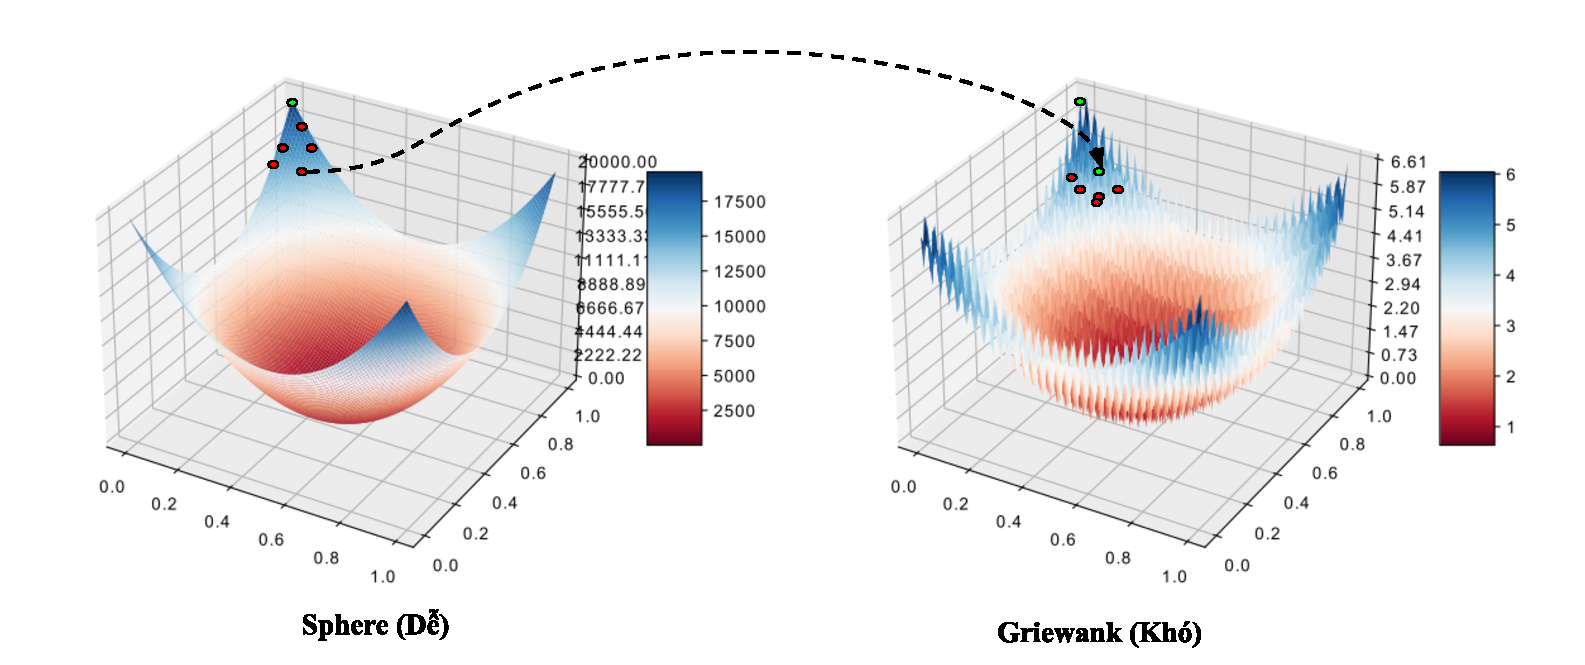
\includegraphics[width=\linewidth]{figure/propose/sequential-motivation.eps}
            \caption{Cập nhật tuần tự trên hai tác vụ có địa hình hàm mục tiêu tương đồng. Trục tung, trục hoành là giá trị của nghiệm. Trục thẳng đứng là giá trị hàm mục tiêu.}
            \label{fig:propsoe:sequential-motivation}
        \end{figure}
    \end{block}
\end{frame}

\begin{frame}{Tóm tắt đóng góp}
    Tóm tắt những ý tốt xấu so với các nghiên cứu liên quan
\end{frame}

\begin{frame}{Áp dụng - Tối ưu nhiều mạng nơ-ron}
    Tổng kết vào đây.
\end{frame}

% \begin{frame}{Task selection as a Multi Armed Bandit (MAB) problem}
%     \begin{block}{Given}
%         \begin{itemize}
%             \item A $K$-task MTO problem
%         \end{itemize}
%     \end{block}
%     \begin{mydef}[Action]
%         For a task $k$, there are $K-1$ actions of choosing $k'$ such that $k' \in \{1, \ldots, K\} \text{ and } k' \ne k$.
%         \label{def:action}
%     \end{mydef}
%     \begin{mydef}[Reward]
%         After task $k'$ is selected to be combined with task $k$, the reward of choosing that action is defined as 
%         \begin{equation}
%             reward = \left\{
%                 \begin{array}{ll}
%                     1 \text{ if } f_k(c) < f_k(p) , \exists p \in P_k \\\
%                     0 \text{ otherwise}.
%                 \end{array}
%               \right.
%         \end{equation}
%         where $c$ is the offspring generated by the reproduction procedure and $f_k(.)$ is the fitness function of the $k^{th}$ task.
%         \label{def:reward}
%     \end{mydef}
% \end{frame}

% \begin{frame}{UCB function to solve MAB}
%     \begin{block}{Property of reward function}
%         \begin{itemize}
%             \item Reward takes two value $0$ or $1$ $\rightarrow$ reward distribution is generated from an unknown Bernoulli distribution.
%             \item From \footfullcite{lattimore2020bandit}, use KL-UCB to solve.
%         \end{itemize}
%     \end{block}
%     \begin{block}{KL-UCB function}
%         \begin{equation}
%             k' = \underset{j}{\text{argmin }} \mu(j) + \frac{1 + t \times log^2(t) }{N(j)}
%             \label{eq:klucb}
%         \end{equation}
%         where 
%         \begin{itemize}
%             \item $\mu(j)$ is the mean of reward when task $j$ is chosen
%             \item $N(j)$ is the number of times task $j$ is chosen
%             \item $t$ is the total number of actions chosen.
%         \end{itemize}
%     \end{block}
% \end{frame}

% \begin{frame}{\gls{propose}, optimize 1 task, 1 generation}
%     \begin{algorithm}[H]
%         \fontsize{6pt}{10}\selectfont
%         \caption{\fontsize{6pt}{10}\selectfont\gls{propose} on each generation of $k^{th}$ task}
%         \begin{algorithmic}[1]
%             \State Initialize $P^{(c)}_k=\emptyset$;
%             \While{number of offspring $< N$}
%                 \State Randomly select $p_a$ from $P_k$;
%                 \If{$rand(0, 1) < rmp$}
%                     \State Choose $k'$ using Formula \eqref{eq:klucb};
%                     \State Randomly select $p_b$ from $P_{k'}$;
%                     \State $c = $ \emph{Inter-task crossover} between  $p_a$ and $p_b$;
%                 \Else
%                     \State Sample $p_b$ from $P_k$;
%                     \State $c = $ \emph{Intra-task crossover} between  $p_a$ and $p_b$;
%                 \EndIf
%                 \State $c = mutate(c)$;
%                 \State Evaluate offspring $c$;
%                 \State Update estimation $\mu(k')$ and $N(k')$ for \gls{klucb} if $c$ generated by inter-task crossover;
%                 \State $P_k^{(c)} = P_c \cup \{c\}$;
%             \EndWhile
%             \State $P_k \leftarrow$ Select $N$ best individuals from $P_k \cup P_k^{(c)}$ to form the next-population of task $k$;
%         \end{algorithmic}
%     \end{algorithm}
% \end{frame}


% \begin{frame}{\gls{propose}, proposed structure for manytasking}
%     \begin{algorithm}[H]
%         \caption{Pseudo code of \gls{propose}}
%         \begin{algorithmic}[1]
%             \For{$k \in \{1, \ldots, K\}$}
%                 \State Randomly sample $N$ individuals to form subpopulation $P_k$;
%                 \State Evaluate individual in $P_k$ for task $k$ only;
%             \EndFor
%             \While{stopping conditions are not satisfied}
%                 \For{$k \in random\_permutation({1, \ldots, K})$}
%                     \State Invoke Algorithm 1 for task $k$;
%                 \EndFor
%             \EndWhile
%         \end{algorithmic}
%     \end{algorithm}
% \end{frame}
